%==============================================================================
% tento soubor pouzijte jako zaklad
% this file should be used as a base for the thesis
% Autoři / Authors: 2008 Michal Bidlo, 2018 Jaroslav Dytrych
% Kontakt pro dotazy a připomínky: dytrych@fit.vutbr.cz
% Contact for questions and comments: dytrych@fit.vutbr.cz
%==============================================================================
% kodovani: UTF-8 (zmena prikazem iconv, recode nebo cstocs)
% encoding: UTF-8 (you can change it by command iconv, recode or cstocs)
%------------------------------------------------------------------------------
% zpracování / processing: make, make pdf, make clean
%==============================================================================
% Soubory, které je nutné upravit: / Files which have to be edited:
%   projekt-20-literatura-bibliography.bib - literatura / bibliography
%   projekt-01-kapitoly-chapters.tex - obsah práce / the thesis content
%   projekt-30-prilohy-appendices.tex - přílohy / appendices
%==============================================================================
\documentclass[slovak,zadani]{fitthesis} % bez zadání - pro začátek práce, aby nebyl problém s překladem
%\documentclass[english]{fitthesis} % without assignment - for the work start to avoid compilation problem
%\documentclass[zadani]{fitthesis} % odevzdani do wisu a/nebo tisk s barevnými odkazy - odkazy jsou barevné
%\documentclass[english,zadani]{fitthesis} % for submission to the IS FIT and/or print with color links - links are color
%\documentclass[zadani,print]{fitthesis} % pro černobílý tisk - odkazy jsou černé
%\documentclass[english,zadani,print]{fitthesis} % for the black and white print - links are black
%\documentclass[zadani,cprint]{fitthesis} % pro barevný tisk - odkazy jsou černé, znak VUT barevný
%\documentclass[english,zadani,cprint]{fitthesis} % for the print - links are black, logo is color
% * Je-li práce psaná v anglickém jazyce, je zapotřebí u třídy použít 
%   parametr english následovně:
%   If thesis is written in english, it is necessary to use 
%   parameter english as follows:
%      \documentclass[english]{fitthesis}
% * Je-li práce psaná ve slovenském jazyce, je zapotřebí u třídy použít 
%   parametr slovak následovně:
%   If the work is written in the Slovak language, it is necessary 
%   to use parameter slovak as follows:
%      \documentclass[slovak]{fitthesis}
% * Je-li práce psaná v anglickém jazyce se slovenským abstraktem apod., 
%   je zapotřebí u třídy použít parametry english a enslovak následovně:
%   If the work is written in English with the Slovak abstract, etc., 
%   it is necessary to use parameters english and enslovak as follows:
%      \documentclass[english,enslovak]{fitthesis}

% Základní balíčky jsou dole v souboru šablony fitthesis.cls
% Basic packages are at the bottom of template file fitthesis.cls
% zde můžeme vložit vlastní balíčky / you can place own packages here

% Kompilace po částech (rychlejší, ale v náhledu nemusí být vše aktuální)
% Compilation piecewise (faster, but not all parts in preview will be up-to-date)
% \usepackage{subfiles}

% Nastavení cesty k obrázkům
% Setting of a path to the pictures
%\graphicspath{{obrazky-figures/}{./obrazky-figures/}}
%\graphicspath{{obrazky-figures/}{../obrazky-figures/}}

%---rm---------------
\renewcommand{\rmdefault}{lmr}%zavede Latin Modern Roman jako rm / set Latin Modern Roman as rm
%---sf---------------
\renewcommand{\sfdefault}{qhv}%zavede TeX Gyre Heros jako sf
%---tt------------
\renewcommand{\ttdefault}{lmtt}% zavede Latin Modern tt jako tt

% vypne funkci šablony, která automaticky nahrazuje uvozovky,
% aby nebyly prováděny nevhodné náhrady v popisech API apod.
% disables function of the template which replaces quotation marks
% to avoid unnecessary replacements in the API descriptions etc.
\csdoublequotesoff

% =======================================================================
% balíček "hyperref" vytváří klikací odkazy v pdf, pokud tedy použijeme pdflatex
% problém je, že balíček hyperref musí být uveden jako poslední, takže nemůže
% být v šabloně
% "hyperref" package create clickable links in pdf if you are using pdflatex.
% Problem is that this package have to be introduced as the last one so it 
% can not be placed in the template file.
\ifWis
\ifx\pdfoutput\undefined % nejedeme pod pdflatexem / we are not using pdflatex
\else
  \usepackage{color}
  \usepackage[unicode,colorlinks,hyperindex,plainpages=false,pdftex]{hyperref}
  \definecolor{hrcolor-ref}{RGB}{223,52,30}
  \definecolor{hrcolor-cite}{HTML}{2F8F00}
  \definecolor{hrcolor-urls}{HTML}{092EAB}
  \hypersetup{
	linkcolor=hrcolor-ref,
	citecolor=hrcolor-cite,
	filecolor=magenta,
	urlcolor=hrcolor-urls
  }
  \def\pdfBorderAttrs{/Border [0 0 0] }  % bez okrajů kolem odkazů / without margins around links
  \pdfcompresslevel=9
\fi
\else % pro tisk budou odkazy, na které se dá klikat, černé / for the print clickable links will be black
\ifx\pdfoutput\undefined % nejedeme pod pdflatexem / we are not using pdflatex
\else
  \usepackage{color}
  \usepackage[unicode,colorlinks,hyperindex,plainpages=false,pdftex,urlcolor=black,linkcolor=black,citecolor=black]{hyperref}
  \definecolor{links}{rgb}{0,0,0}
  \definecolor{anchors}{rgb}{0,0,0}
  \def\AnchorColor{anchors}
  \def\LinkColor{links}
  \def\pdfBorderAttrs{/Border [0 0 0] } % bez okrajů kolem odkazů / without margins around links
  \pdfcompresslevel=9
\fi
\fi
% Řešení problému, kdy klikací odkazy na obrázky vedou za obrázek
% This solves the problems with links which leads after the picture
\usepackage[all]{hypcap}

% Informace o práci/projektu / Information about the thesis
%---------------------------------------------------------------------------
\projectinfo{
  %Prace / Thesis
  project={BP},            %typ práce BP/SP/DP/DR  / thesis type (SP = term project)
  year={2019},             % rok odevzdání / year of submission
  date=\today,             % datum odevzdání / submission date
  %Nazev prace / thesis title
  title.cs={Aplikace na podporu výuky dynamického programování},  % název práce v češtině či slovenštině (dle zadání) / thesis title in czech language (according to assignment)
  title.en={Application for the Dynamic Programming Demonstration}, % název práce v angličtině / thesis title in english
  %title.length={14.5cm}, % nastavení délky bloku s titulkem pro úpravu zalomení řádku (lze definovat zde nebo níže) / setting the length of a block with a thesis title for adjusting a line break (can be defined here or below)
  %Autor / Author
  author.name={Tomáš},   % jméno autora / author name
  author.surname={Nereča},   % příjmení autora / author surname 
  %author.title.p={Bc.}, % titul před jménem (nepovinné) / title before the name (optional)
  %author.title.a={Ph.D.}, % titul za jménem (nepovinné) / title after the name (optional)
  %Ustav / Department
  department={UIFS}, % doplňte příslušnou zkratku dle ústavu na zadání: UPSY/UIFS/UITS/UPGM / fill in appropriate abbreviation of the department according to assignment: UPSY/UIFS/UITS/UPGM
  % Školitel / supervisor
  supervisor.name={Ivana},   % jméno školitele / supervisor name 
  supervisor.surname={Burgetová},   % příjmení školitele / supervisor surname
  supervisor.title.p={Ing.},   %titul před jménem (nepovinné) / title before the name (optional)
  supervisor.title.a={Ph.D.},    %titul za jménem (nepovinné) / title after the name (optional)
  % Klíčová slova / keywords
  keywords.cs={DP, Dynamické programovanie, algoritmy, rekurzia, react, typescript \todo{doplnit}}, % klíčová slova v českém či slovenském jazyce / keywords in czech or slovak language
  keywords.en={DP, Dynamic programming, \todo{doplnit}}, % klíčová slova v anglickém jazyce / keywords in english
  %keywords.en={Here, individual keywords separated by commas will be written in English.},
  % Abstrakt / Abstract
  abstract.cs={Optimalizačná technika - dynamické programovanie môže byť pri určitom type úloh veľmi efektívna. Webová aplikácia, ktorá je predmetom tejto bakalárskej práce na sérii praktických príkladov pomocou grafickej vizualizácie vysvetluje príncipy dynamického programovania. Ku každému príkladu poskytuje potrebnú teóriu k pochopeniu fungovania algoritmu. Okrem toho aplikácia porovnáva efektivitu riešenia technikou dynamického programovania s rekurzívnym riešením zakreslovaním štatistík do grafov a tabuliek. Aplikácia má slúžiť ako podpora pri výučbe dynamického programovania.}, % abstrakt v českém či slovenském jazyce / abstract in czech or slovak language
  abstract.en={\todo{doplnit}}, % abstrakt v anglickém jazyce / abstract in english
  %abstract.en={An abstract of the work in English will be written in this paragraph.},
  % Prohlášení (u anglicky psané práce anglicky, u slovensky psané práce slovensky) / Declaration (for thesis in english should be in english)
  declaration={Prehlasujem, že som túto bakalársku prácu vypracoval samostatne pod vedením Ing. Ivany Burgetovej  Ph.D.
Uviedol som všetky literárne pramene a publikácie, z ktorých som čerpal.},
  %declaration={Hereby I declare that this bachelor's thesis was prepared as an original author’s work under the supervision of Mr. X
% The supplementary information was provided by Mr. Y
% All the relevant information sources, which were used during preparation of this thesis, are properly cited and included in the list of references.},
  % Poděkování (nepovinné, nejlépe v jazyce práce) / Acknowledgement (optional, ideally in the language of the thesis)
  acknowledgment={Rád by som poďakoval Ing. Ivane Burgetovej  Ph.D. za cenné rady, pripomienky a trpezlivosť pri vedení mojej bakalárskej práce.},
  %acknowledgment={Here it is possible to express thanks to the supervisor and to the people which provided professional help
%(external submitter, consultant, etc.).},
  % Rozšířený abstrakt (cca 3 normostrany) - lze definovat zde nebo níže / Extended abstract (approximately 3 standard pages) - can be defined here or below
  %extendedabstract={Do tohoto odstavce bude zapsán rozšířený výtah (abstrakt) práce v českém (slovenském) jazyce.},
  %faculty={FIT}, % FIT/FEKT/FSI/FA/FCH/FP/FAST/FAVU/USI/DEF
  faculty.cs={Fakulta informačních technologií}, % Fakulta v češtině - pro využití této položky výše zvolte fakultu DEF / Faculty in Czech - for use of this entry select DEF above
  faculty.en={Faculty of Information Technology}, % Fakulta v angličtině - pro využití této položky výše zvolte fakultu DEF / Faculty in English - for use of this entry select DEF above
  department.cs={Ústav informačních systémů}, % Ústav v češtině - pro využití této položky výše zvolte ústav DEF nebo jej zakomentujte / Department in Czech - for use of this entry select DEF above or comment it out
  department.en={Department of Information Systems} % Ústav v angličtině - pro využití této položky výše zvolte ústav DEF nebo jej zakomentujte / Department in English - for use of this entry select DEF above or comment it out
}

% Rozšířený abstrakt (cca 3 normostrany) - lze definovat zde nebo výše / Extended abstract (approximately 3 standard pages) - can be defined here or above
%\extendedabstract{Do tohoto odstavce bude zapsán výtah (abstrakt) práce v českém (slovenském) jazyce.}

% nastavení délky bloku s titulkem pro úpravu zalomení řádku - lze definovat zde nebo výše / setting the length of a block with a thesis title for adjusting a line break - can be defined here or above
%\titlelength{14.5cm}


% řeší první/poslední řádek odstavce na předchozí/následující stránce
% solves first/last row of the paragraph on the previous/next page
\clubpenalty=10000
\widowpenalty=10000

% checklist
\newlist{checklist}{itemize}{1}
\setlist[checklist]{label=$\square$}

\usepackage{amsthm}
\usepackage{listings}
\newtheorem{example}{Príklad}

\begin{document}
  % Vysazeni titulnich stran / Typesetting of the title pages
  % ----------------------------------------------
  \maketitle
  % Obsah
  % ----------------------------------------------
  \setlength{\parskip}{0pt}

  {\hypersetup{hidelinks}\tableofcontents}
  
  % Seznam obrazku a tabulek (pokud prace obsahuje velke mnozstvi obrazku, tak se to hodi)
  % List of figures and list of tables (if the thesis contains a lot of pictures, it is good)
  \ifczech
    \renewcommand\listfigurename{Seznam obrázků}
  \fi
  \ifslovak
    \renewcommand\listfigurename{Zoznam obrázkov}
  \fi
  % \listoffigures
  
  \ifczech
    \renewcommand\listtablename{Seznam tabulek}
  \fi
  \ifslovak
    \renewcommand\listtablename{Zoznam tabuliek}
  \fi
  % \listoftables 

  \ifODSAZ
    \setlength{\parskip}{0.5\bigskipamount}
  \else
    \setlength{\parskip}{0pt}
  \fi

  % vynechani stranky v oboustrannem rezimu
  % Skip the page in the two-sided mode
  \iftwoside
    \cleardoublepage
  \fi

  % Text prace / Thesis text
  % ----------------------------------------------
  %===============================================================================
% Autoři: Michal Bidlo, Bohuslav Křena, Jaroslav Dytrych, Petr Veigend a Adam Herout 2018

\chapter{Úvod}
Bežný človek musí dennodenne riešiť rôzne typy úloh. Niektoré sú jednoduchšie, ako napríklad vyniesť odpadky, niektoré naopak zložitejšie, napríklad z pracovného prostredia. Cieľom každého z nás by malo byť efektívne riešenie týchto úloh. Informačné systémy riešia úlohy pomocou vopred definovaných postupov. Je rovnako dôležité aby aj tieto postupy boli dobre optimalizované. 

Dynamické programovanie (skrátene DP) \footnote{\textbf{DP} je často používaná skratka pre \textbf{D}ynamické \textbf{P}rogramovanie. Bude používaná aj v ďalším kapitolách tejto práce.} je optimalizačná metóda, ktorá môže podstatne zrýchliť výpočet určitého typu úloh. Princípom je ukladanie podvýsledkov, ktoré by inak boli vypočítavané znovu a znovu.

Moderná webová aplikácia, ktorá je výsledkom tejto práce vysvetľuje túto metódu na sérii príkladov. Používateľ aplikácie si môže sám zvoliť vstupné hodnoty a sledovať priebeh výpočtu. Okrem toho aplikácia vykresľuje aj grafy a tabuľky pre porovnanie štatistík pri jednoduchom riešení a pri využití dynamického programovania. Týmto sa líši od voľne dostupných webových prezentácií, ktoré síce poskytujú teóriu a riešenia veľkého počtu príkladov, ale neponúkajú grafické znázornenie princípu jednotlivých algoritmov.

Aplikácia má slúžiť hlavne ako podporný materiál pri výučbe. Využitie teda nájde najmä v akademickej sfére, ale zaujímavá môže byť pre každého kto sa aspoň trochu zaujíma o programovanie, algoritmy alebo aj matematické výpočty.

Následujúca kapitola tejto práce obsahuje nevyhnutnú teóriu k pochopenie princípov dynamického programovania, kedy je možné túto metódu použiť a aké výhody prináša. 

3. kapitola sa sústredí na návrh aplikácie. To zahŕňa výber technológií, návrh užívateľského rozhrania a štruktúry aplikácie. 

4. kapitola popisuje konkrétnu implementáciu. 5. kapitola sa zaoberá testovaním. Uvedené postrehy od študentov ale aj od bežných užívateľov, ktoré boli veľmi užitočné pre ladenie aplikácie.

Záverečná kapitola obsahuje zhrnutie výsledkov práce a ponúka možnosti na ďalšie vylepšenie a rozšírenie aplikácie.



\chapter{Dynamické programovanie}
\label{dynamickeProgramovanie}

V tejto kapitole sú preberané princípy optimalizačnej metódy -- dynamického programovania. Úvod kapitoly je zameraný na hlavné myšlienky tejto metódy, a teda rozdelenie úlohy na podproblémy a ukladanie dielčich výsledkov výpočtu. Z toho vyplývajú podmienky, ktoré musí naivné riešenie danej úlohy spĺňať aby sa miesto neho dalo použiť dynamické programovanie. Ďalej budú preberané konkrétne úlohy, ktoré sú súčasťou aplikácie. 

\section{Hlavné princípy dynamického programovania}

Dynamické programovanie je optimalizačná metóda, ktorá sa dá využiť pri riešení optimalizačných úloh \footnote{Optimalizačná úloha, je úloha, ktorá má viacero správnych riešení. Každé z týchto riešení má určitú hodnotu. Cieľom je nájsť extrém (najnižšiu alebo najvyššiu hodnotu). Riešení ktorých výsledkom je extrém môže byť viacero. Môže teda existovať viacero optimálnych riešení.\cite{IntroductionToAlg}}. Okrem oblasti informatiky sa s dynamickým programovaním môžme stretnúť napríklad aj v matematike. Názov tejto metódy môže byť preto trochu mätúci. Slovo \uv{programovanie} by malo poukazovať na \textbf{tabuľkovú metódu}.

Hlavným princípom metódy je dynamické ukladanie podvýsledkov do dátovej štruktúry (poľa alebo práve tabuľky), ktorých spojením sa dá určiť hodnota optimálneho riešenia, prípadne skonštruovať celé riešenie. Využíva rekurzívny rozklad problému na podproblémy \todo{labyrint algoritmu str.283}, podobne ako metóda \uv{Rozdeľuj a panuj}\todo{nieco k metode}. Jej výhoda ale spočíva práve v tom, že využíva opakovanie podproblémov a preto vedie často k oveľa rýchlejšiemu riešeniu.

Z týchto skutočností vyplývajú 2 podmienky nutné k tomu, aby daná úloha mohla byť riešená dynamickým programovaním:

\begin{enumerate}
    \item \textbf{Prekrývajúce sa podproblémy} \ref{prekryvPodProb}
    \item \textbf{Optimálna subštruktúra} \ref{optimalSubstrukt}
\end{enumerate}

\subsection{Prekrývanie podproblémov} \label{prekryvPodProb}
Ak sa pri riešení úlohy opakujú rovnaké podproblémy, je to prvým znamením, ktoré nabáda k využitiu dynamického programovania. Zistiť, či sa pri riešení úlohy vyskytujú podproblémy, ktorých výsledky sú vypočítavané viacnásobne sa dá zistiť jednoducho zakreslením \textbf{stromu rekurzie} \ref{stromRekurzie}.

\begin{figure} \label{stromRekurzie}
  \caption{Strom rekurzie graficky znázorňuje priebeh rekurzívneho riešenia úlohy. Pri uzloch vyznačených rovnakou farbou ide o rovnaké podproblémy, ktoré sú vypočítavané viacnásobne.}
  \centering
    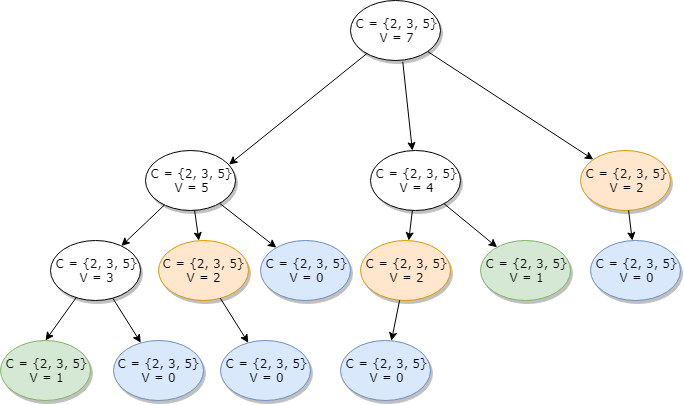
\includegraphics[width=0.8\textwidth]{obrazky-figures/coinsTree.png}
\end{figure}

Ak je zrejmé, že podproblémy sa neopakujú, použiť dynamické programovanie nemá zmysel. Práve naopak. Pri dynamickom programovaní by sa iba zvýšila \textbf{priestorová zložitosť} \todo{co je to} algoritmu z dôvodu vytvorenia dátovej štruktúry na ukladanie podvýsledkov. 

\subsection{Optimálna subštruktúra} \label{optimalSubstrukt}
Druhou vlastnosťou, ktorú musí optimalizačná úloha spĺňať sa nazýva \textbf{optimálna subštruktúra}. V prvom rade sa musí dať úloha rozdeliť na podproblémy. Každý z týchto podproblémov má vlastné optimálne riešenie. Ak sa spojením týchto čiastkových riešení dá dostať optimálne riešenie celej úlohy, dá sa konštatovať, že úloha má optimálnu subštruktúru. \cite{IntroductionToAlg}

\section{Vytvorenie algoritmu využívajúceho dynamické programovanie}

Vytvorenie efektívneho algoritmu postaveného na princípoch dynamického programovania zahŕňa obvykle 4 kroky:

\begin{enumerate}
    \item \textbf{Charakterizovanie štruktúry optimálneho riešenia úlohy} \ref{charakterStrukt}
    \item \textbf{Definovanie hodnoty optimálneho riešenia úlohy pomocou rekurzie} \ref{defOptRies}
    \item \textbf{Výpočet hodnoty optimálneho riešenia pomocou tabuľkovej metódy} \ref{vypocetHodnoty}
    \item \textbf{Zostavenie optimálneho riešenia s využitím vypočítaných hodnôt} \ref{zostavRies}
\end{enumerate}

Kroky 1.-3. je potrebné vykonať vždy. 4. krok je potrebný v prípade, ak je potrebné okrem hodnoty optimálneho riešenia zostaviť aj celé riešenie. Všetky kroky budú vysvetlené na nasledujúcom príklade, ktorý je aj súčasťou výslednej aplikácie: 

\begin{example}
%\textnormal{\textbf{Minimálny počet mincí na vytvorenie danej hodnoty}}
Majme neobmedzený počet mincí rôznych hodnôt $C=(c1, c2, c3, ..., cN)$ a hodnotu, ktorá má vzniknúť súčtom hodnôt mincí. Pre súčet musí byť využitý čo najmenší počet mincí. Ktoré mince budú použité a aký je ich počet?
\end{example}

\subsection{Charakterizovanie štruktúry optimálneho riešenia úlohy} \label{charakterStrukt}

V prvom kroku je potrebné danú optimalizačnú úlohu analyzovať. Dôležité je určiť si jednoduché vstupné hodnoty, aby sa dalo k optimálnemu riešeniu dostať stratégiou \uv{pokus--omyl}. Budú sa teda testovať kombinácie všetkých možných hodnôt, až nakoniec vypadne najoptimálnejšia kombinácia alebo aj viacero kombinácií s rovnakou výslednou hodnotou. Pri tomto naivnom zisťovaní výsledku sa dajú vyvodiť potrebné informácie, ktoré potvrdia alebo vyvrátia podmienky potrebné k tomu aby sa dal vytvoriť DP algoritmus.

\bigskip 

\noindent Určíme si vstupné hodnoty úlohy: 
\begin{itemize}
    \item Mince: 1, 2, 3, 5
    \item Hodnota: 8
\end{itemize}

Na prvý pohľad je jasné, že riešením je použiť 8 mincí s hodnotou 1, ale toto riešenie by nebolo optimálne. Skúsime teda použiť mincu s hodnotou 2. Aby sme v súčte dostali hodnotu 8, musíme pridať ďalšie 3 mince s hodnotou 2, prípadne použiť mincu s hodnotou 5 a pridať ešte mincu s hodnotou 1. Vypíšme si teda niektoré riešenia úlohy:

\begin{itemize}
    \item 2 + 2 + 2 + 2 = 8
    \item 2 + 2 + 3 + 1 = 8
    \item 2 + 3 + 3 = 8
    \item 3 + 2 + 2 + 1 = 8
    \item 5 + 2 + 1 = 8
    \item 5 + 3 = 8
\end{itemize}

Ak vyberieme mincu s hodnotou 2, musíme ďalej riešiť podproblém, kedy potrebujeme získať v súčet 6. Pridáme napríklad mincu s hodnotou 3. Ďalší podproblém bude získať súčet 3. Ten môžeme získať pridaním jednej mince s hodnotou 3 alebo mincí s hodnotami 2 a 1. Optimálne je vybrať minci s hodnotou 3. Takto nám vznikajú podproblémy, ktoré je možné riešiť nezávisle , a ktorých optimálnym riešením získame aj optimálne riešenie pôvodnej úlohy. Tým sme dokázali, že riešenie úlohy má \textbf{optimálnu subštruktúru}.

Pri tomto konkrétnom zadaní môže byť optimálne riešenie jasné. Je ním posledné riešenie, a teda súčet mincí s hodnotami 5 a 3. Minimálny počet mincí je teda 2. Problém by nastal pri zadaní viacerých typov mincí a vyššej hodnoty. Ďalším krokom je teda vytvorenie algoritmu. 

Pozn.: Okrem optimálneho riešenia si môžeme všimnúť, že niektoré podproblémy sú riešené viacnásobne, čo sa nám aj potvrdí po navrhnutí rekurzívneho algoritmu.

\subsection{Definovanie hodnoty optimálneho riešenia úlohy pomocou rekurzie} \label{defOptRies}

Po charakterizovaní štruktúry optimálneho riešenia vzhľadom na podproblémy nasleduje 2. krok. Ten spočíva v návrhu rekurzívneho algoritmu, využijeme teda metódu \uv{Zhora dole} \footnote{\textbf{Zhora dole} je metóda návrhu algoritmu. Princípom je postupné rozkladanie riešenia na jednoduchšie operácie až k elementárnym krokom.} k vytvoreniu formuly. Ako vzor poslúži opäť príklad s mincami. 

V prvom rade vezmeme do úvahy špecifický prípad, od ktorého sa odrazíme. Ak je zadaná hodnota rovná 0, aj počet mincí bude 0. Ak je hodnota väčšia ako 0, zoberieme postupne všetky mince, ktorých hodnota je menšia alebo rovná požadovanej hodnote. Od požadovanej hodnoty sa odpočíta hodnota mince a rekurzívne sa zavolá rovnaká metóda pre túto novú požadovanú hodnotu, pričom sa inkrementuje počet použitých mincí. Riešenie možno popísať formulou (kód v jazyku C je v prílohe):

$$
minMince(m[0..p - 1], h) = min
\left\{
\begin{array}{ll}
1 + minMince(m, h - m[i]) &\ \text{kde}\ 0 \leq i \leq p - 1\\
0 &\ \text{ak}\ h=0
\end{array}
\right.
$$

\begin{itemize}
    \item m - zadané mince
    \item p - počet mincí
    \item h - zadaná hodnota
\end{itemize}

Kód v jazyku C:



\subsection{Výpočet hodnoty optimálneho riešenia pomocou tabuľkovej metódy} \label{vypocetHodnoty}
\subsection{Zostavenie optimálneho riešenia s využitím vypočítaných hodnôt} \label{zostavRies}

\subsection{Rekonštrukcia optimálneho riešenia úlohy}

\section{Optimalizačné úlohy riešiteľné dynamickým programovaním}
\subsection{Minimálny počet mincí na vytvorenie danej hodnoty}
\subsection{Problém rezania tyče}
\subsection{Najdlhší spoločný podreťazec}
\subsection{Editačná vzdialenosť}
\subsection{Optimalizovaný binárny vyhľadávací strom}

\chapter{Návrh webovej aplikácie} 
\label{navrhAplikacie}
\section{Webové stránky so zameraním na dynamické programovanie - súčasný stav}
\section{Požiadavky kladené na novú webovú aplikáciu}
\section{Výber technológií pre vytvorenie modernej webovej aplikácie}
\subsection{React}
\subsection{Typescript}
\section{Návrh užívateľského rozhrania}
\subsection{Rozdelenie do kontajnerov}
\subsection{Teória}
\subsection{Demo}
\subsection{Grafy}

\chapter{Implementácia}
\label{implementacia}
\section{Štruktúra zdrojových textov}
\section{Zapúzdrenie do komponent}
\section{Hlavné časti aplikácie }
\subsection{Teória}
\todo{Zobrazenie zdrojových textov}
\subsection{Demo}
\todo{Vykresľovanie tabuľky}
\subsection{Grafy}
\todo{Vykresľovanie grafov}
\todo{Počítanie štatistik}

\chapter{Testovanie}
\label{testovanie}
\section{Testovací scenár}
\section{Testovanie s používateľmi}
\section{Vyhodnotenie testov}
\section{Úpravy aplikácie}

\chapter{Zaver}
\label{zaver}
  
  % Kompilace po částech (viz výše, nutno odkomentovat)
  % Compilation piecewise (see above, it is necessary to uncomment it)
  %\subfile{projekt-01-uvod-introduction}
  % ...
  %\subfile{chapters/projekt-05-conclusion}


  % Pouzita literatura / Bibliography
  % ----------------------------------------------
\ifslovak
  \makeatletter
  \def\@openbib@code{\addcontentsline{toc}{chapter}{Literatúra}}
  \makeatother
  \bibliographystyle{bib-styles/slovakiso}
\else
  \ifczech
    \makeatletter
    \def\@openbib@code{\addcontentsline{toc}{chapter}{Literatura}}
    \makeatother
    \bibliographystyle{bib-styles/czechiso}
  \else 
    \makeatletter
    \def\@openbib@code{\addcontentsline{toc}{chapter}{Bibliography}}
    \makeatother
    \bibliographystyle{bib-styles/englishiso}
  %  \bibliographystyle{alpha}
  \fi
\fi
  \begin{flushleft}
  \bibliography{projekt-20-literatura-bibliography}
  \end{flushleft}

  % vynechani stranky v oboustrannem rezimu
  % Skip the page in the two-sided mode
  \iftwoside
    \cleardoublepage
  \fi

  % Prilohy / Appendices
  % ---------------------------------------------
  \appendix
\ifczech
  \renewcommand{\appendixpagename}{Přílohy}
  \renewcommand{\appendixtocname}{Přílohy}
  \renewcommand{\appendixname}{Příloha}
\fi
\ifslovak
  \renewcommand{\appendixpagename}{Prílohy}
  \renewcommand{\appendixtocname}{Prílohy}
  \renewcommand{\appendixname}{Príloha}
\fi
%  \appendixpage

% vynechani stranky v oboustrannem rezimu
% Skip the page in the two-sided mode
%\iftwoside
%  \cleardoublepage
%\fi
  
\ifslovak
%  \section*{Zoznam príloh}
%  \addcontentsline{toc}{section}{Zoznam príloh}
\else
  \ifczech
%    \section*{Seznam příloh}
%    \addcontentsline{toc}{section}{Seznam příloh}
  \else
%    \section*{List of Appendices}
%    \addcontentsline{toc}{section}{List of Appendices}
  \fi
\fi
  \startcontents[chapters]
  \setlength{\parskip}{0pt}
  % seznam příloh / list of appendices
  % \printcontents[chapters]{l}{0}{\setcounter{tocdepth}{2}}
  
  \ifODSAZ
    \setlength{\parskip}{0.5\bigskipamount}
  \else
    \setlength{\parskip}{0pt}
  \fi
  
  % vynechani stranky v oboustrannem rezimu
  \iftwoside
    \cleardoublepage
  \fi
  
  % Přílohy / Appendices
  % Tento soubor nahraďte vlastním souborem s přílohami (nadpisy níže jsou pouze pro příklad)
% This file should be replaced with your file with an appendices (headings below are examples only)

% Umístění obsahu paměťového média do příloh je vhodné konzultovat s vedoucím
% Placing of table of contents of the memory media here should be consulted with a supervisor
%\chapter{Obsah přiloženého paměťového média}

%\chapter{Manuál}

%\chapter{Konfigurační soubor} % Configuration file

%\chapter{RelaxNG Schéma konfiguračního souboru} % Scheme of RelaxNG configuration file

%\chapter{Plakát} % poster

\chapter{Minimálny počet mincí na vytvorenie danej hodnoty - rekurzívne riešenie v jazyku C}
\begin{lstlisting}
// Returns number of coins to make given value
// coins[] - array of different coin types
// arrSize - size of array coins[]
// value - value we need to make
int minCoins(int coins[], int arrSize, int value) 
{
    // Base case
    if (value == 0)
    {
        return 0;
    }

    // Initialize result
    int res = INT_MAX; // From limits.h

    // Loop trough all coins smaller or equal to given value
    for (int i = 0; i < arrSize; i++)
    {
        if (coins[i] <= value) 
        { 
            int subRes = minCoins(coins, arrSize, value - coins[i]);

            // Check for INT_MAX to avoid overflow and see 
            // if result can be minimized
            if (subRes != INT_MAX && subRes + 1 < res)
            {
                res = subRes + 1;
            }
        }
    }
    return res;
}
\end{lstlisting}


  
  % Kompilace po částech (viz výše, nutno odkomentovat)
  % Compilation piecewise (see above, it is necessary to uncomment it)
  %\subfile{projekt-30-prilohy-appendices}
  
\end{document}
